% Observation-clock and impact supplement insert for v2.1.0.

\subsection{Mittag--Leffler renewal clocks}
\label{app:mittag-leffler-clocks}

Let $W_{\beta,\tau}$ denote a positive Mittag--Leffler waiting interval.  The
implemented convention is fixed by its Laplace transform,
\begin{equation}
\mathbb E[e^{-sW_{\beta,\tau}}]
=\frac{1}{1+(\tau s)^\beta},
\qquad 0<\beta\leq1,\quad \tau>0.
\label{eq:ml-wait-laplace}
\end{equation}
For $0<\beta<1$ it has infinite mean.  If $E$ is unit exponential and
$S_\beta$ is positive stable with
$\mathbb E[e^{-sS_\beta}]=e^{-s^\beta}$, the sampler uses
$W_{\beta,\tau}=\tau E^{1/\beta}S_\beta$.  The positive-stable draw uses the
Kanter representation in Algorithm~\ref{alg:renewal-clock-construction}.

Exponential tempering is defined as a probability-law tilt, not by truncating
realised waits.  For rate $\lambda_T>0$ its transform and mean are
\begin{align}
\mathbb E[e^{-sW^{(T)}_{\beta,\tau}}]
&=\frac{1+(\tau\lambda_T)^\beta}
{1+[\tau(s+\lambda_T)]^\beta},
\label{eq:tempered-ml-laplace}\\
\mathbb E[W^{(T)}_{\beta,\tau}]
&=\frac{\beta\tau^\beta\lambda_T^{\beta-1}}
{1+(\tau\lambda_T)^\beta}.
\label{eq:tempered-ml-mean}
\end{align}
Exact rejection sampling accepts an untempered candidate $w$ with probability
$e^{-\lambda_Tw}$.  Monte Carlo controls over 240,000 supplied candidate
uniform quadruples give maximum Laplace-transform errors $9.76\times10^{-4}$
and $1.03\times10^{-3}$ for the untempered and tempered laws, respectively;
the tempered mean has relative error $2.67\times10^{-3}$.  The 99th-percentile
wait falls from $487.6$ s to $78.2$ s under tempering.  Random-number streams
remain caller-owned and book-specific.

\subsection{Paired price and meta-order impact across clocks}
\label{app:clock-impact}

The implementation audit used Diana and Gebbie's
\href{https://github.com/DerickDiana/InteractingLOBs.jl}{InteractingLOBs.jl}
at commit \texttt{098f1807}.  Its substantive routine
\texttt{src/useful\_functions.jl:calculate\_price\_impacts} measures signed
raw-price displacement after an injected order and aggregates paths; the
repository-root \texttt{plot\_price\_impact.jl} is only a stub.  The associated
method is described in
\href{https://doi.org/10.1016/j.cam.2024.116202}{Diana and Gebbie,
\emph{J. Comput. Appl. Math.} 2024} and arXiv:2310.06079.  The Julia routine is
a methodological reference and is not ported.  The v2.1.0 implementation uses
the common-input shocked-minus-control estimator established in Figures 9 and
10.

For event book $b$, response book $j$, sign $s\in\{-1,+1\}$, path $p$ and
clock domain $c$, the reported single-trade estimand is
\begin{equation}
\widehat I^{(c)}_{b\to j}(\ell)=
\frac{1}{2P}\sum_{p=1}^{P}\sum_{s\in\{-1,+1\}}
s\left[P^{(c),\mathrm{shock}}_{p,j}(t_e+\ell)
-P^{(c),\mathrm{control}}_{p,j}(t_e+\ell)\right].
\label{eq:paired-clock-impact}
\end{equation}
The shocked and control paths use identical initial states and operational
innovations.  For each observation domain they also use the same realised
book clock, so a response can be delayed or held but not generated by a clock
mismatch.  The meta-order estimand applies Eq.~\eqref{eq:paired-clock-impact}
to the declared four-child fast and slow schedules and reports lag from the
last child.  Active-observation fractions are stored with the curves; inactive
paths contribute zero at that calendar query, preserving the unconditional
clock effect.

\begin{figure}[p]
\centering
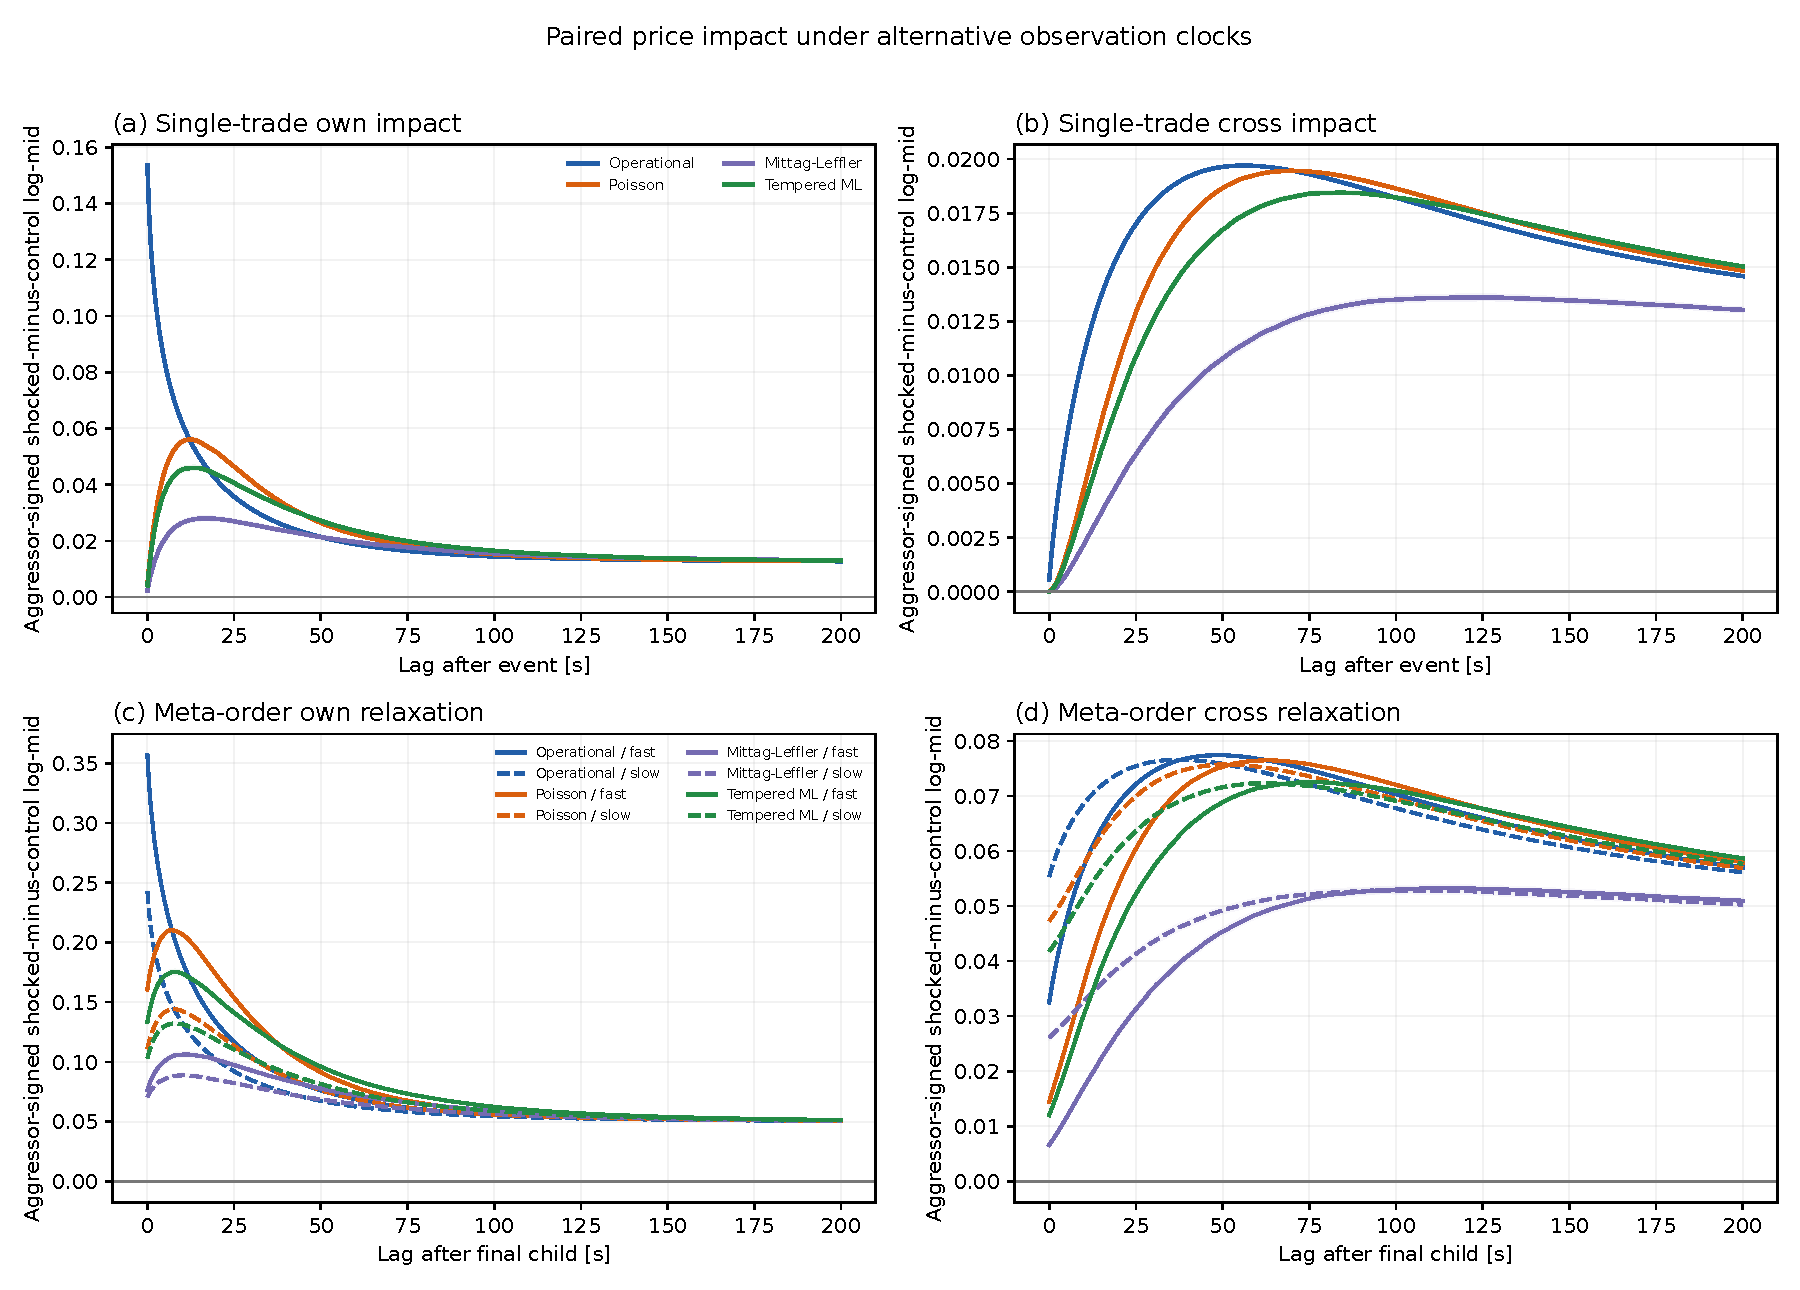
\includegraphics[width=\textwidth]{figures/figure-14-clock-subordinated-impact-v2.pdf}
\caption{\textbf{Paired price impact under alternative observation clocks.}
Panels (a) and (b) report single-trade own and cross impact.  Panels (c) and
(d) report own and cross relaxation after the final child of the fast (solid)
and slow (dashed) meta-order schedules.  Blue, orange, purple and green denote
operational, Poisson, Mittag--Leffler and tempered Mittag--Leffler domains.
The operational response is unchanged across comparisons.  Previous-refresh
observation delays early own impact and cross-impact propagation; untempered
heavy-tailed waits produce the greatest finite-horizon attenuation and
uncertainty, while tempering restores more timely observation.  Long-lag
convergence reflects observation of the same underlying paired paths.  These
are conditional model responses, not empirical impact laws, optimal-execution
curves or fitted power laws.}
\label{fig:clock-subordinated-impact}
\end{figure}
